\documentclass[a4paper,11pt]{report}
\usepackage{chuan_math_gkt}
\usetikzlibrary{angles,quotes,intersections,patterns,decorations.pathreplacing}
\chuanexamsetup

\begin{document}
\examfontsize

\examsecret{绝密$\bigstar$启用前}

\examtitle{2025年普通高等学校招生全国统一考试（天津卷）}{数\quad 学}

\noticetitle
\begin{examnotice}
\item 答卷前，考生务必将自己的姓名、准考证号填写在答题卡上。
\item 回答选择题时，选出每小题的答案后，用铅笔把答题卡上对应题目的答案标号涂黑。如需改动，用橡皮擦干净后，再选涂其他答案标号。回答非选择题时，将答案写在答题卡上。写在本试卷上无效。
\item 考试结束后，将本试卷和答题卡一并交回。
\end{examnotice}

\examsection{一、选择题：本大题共9小题，每小题5分，共45分。在每小题给出的四个选项中，只有一项是符合题目要求的。}
\begin{examquestions}
\item 已知集合 $U=\{1,2,3,4,5\}$，$A=\{1,3\}$，$B=\{2,3,5\}$，则 $\complement_U(A\cup B)=$
\fourchoices{$\{1,2,3,4\}$}{$\{2,3,4\}$}{$\{2,4\}$}{$\{4\}$}

\item 设 $x\in\mathbb R$，则“$x=0$”是“$\sin2x=0$”
\twochoices{充分不必要条件}{必要不充分条件}{充要条件}{既不充分也不必要条件}

\item 已知函数 $y=f(x)$ 的图象如下，则 $f(x)$ 的解析式可能为
\begin{tightcenter}
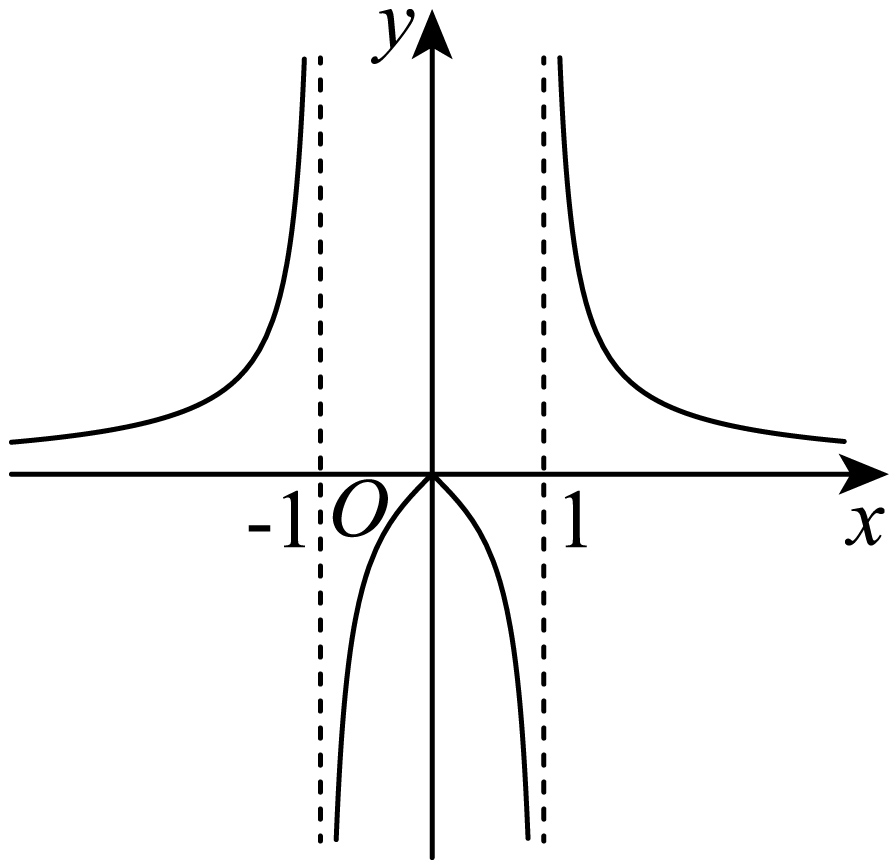
\includegraphics[width=4.0cm]{figures/2025_tj_q3.png}
\end{tightcenter}
\fourchoices{\tallchoice{$f(x)=\dfrac{x}{1-|x|}$}}{\tallchoice{$f(x)=\dfrac{x}{|x|-1}$}}{\tallchoice{$f(x)=\dfrac{|x|}{1-x^2}$}}{\tallchoice{$f(x)=\dfrac{|x|}{x^2-1}$}}

\item 若 $m$ 为直线，$\alpha,\beta$ 为两个平面，则下列结论中正确的是
\onechoices
{若 $m\parallel\alpha$，$n\subset\alpha$，则 $m\parallel n$}
{若 $m\perp\alpha$，$m\perp\beta$，则 $\alpha\perp\beta$}
{若 $m\parallel\alpha$，$m\perp\beta$，则 $\alpha\perp\beta$}
{若 $m\subset\alpha$，$\alpha\perp\beta$，则 $m\perp\beta$}

\item 下列说法中错误的是
\onechoices
{若 $X\sim N(\mu,\sigma^2)$，则 $P(X\leq\mu-\sigma)=P(X\geq\mu+\sigma)$}
{若 $X\sim N(1,2^2)$，$Y\sim N(2,2^2)$，则 $P(X<1)<P(Y<2)$}
{$|r|$ 越接近 $1$，相关性越强}
{$|r|$ 越接近 $0$，相关性越弱}

\item $S_n=-n^2+8n$，则数列 $\{|a_n|\}$ 的前 $12$ 项和为
\fourchoices{$112$}{$48$}{$80$}{$64$}

\item 函数 $f(x)=0.3^x-\sqrt{x}$ 的零点所在区间是
\fourchoices{$(0,0.3)$}{$(0.3,0.5)$}{$(0.5,1)$}{$(1,2)$}

\item $f(x)=\sin(\omega x+\varphi)(\omega>0,-\pi<\varphi<\pi)$，在 $\left[-\dfrac{5\pi}{12},\dfrac{\pi}{12}\right]$ 上单调递增，且 $x=\dfrac{\pi}{12}$ 为它的一条对称轴，$\left(\dfrac{\pi}{3},0\right)$ 是它的一个对称中心，当 $x\in\left[0,\dfrac{\pi}{2}\right]$ 时，$f(x)$ 的最小值为
\fourchoices{\tallchoice{$-\dfrac{\sqrt3}{2}$}}{\tallchoice{$-\dfrac12$}}{$1$}{$0$}

\item 双曲线 $\dfrac{x^2}{a^2}-\dfrac{y^2}{b^2}=1(a>0,b>0)$ 的左、右焦点分别为 $F_1,F_2$，以右焦点 $F_2$ 为焦点的抛物线 $y^2=2px(p>0)$ 与双曲线交于第一象限的点 $P$，若 $|PF_1|+|PF_2|=3|F_1F_2|$，则双曲线的离心率 $e=$
\fourchoices{$2$}{$5$}{\tallchoice{$\dfrac{\sqrt2+1}{2}$}}{\tallchoice{$\dfrac{\sqrt5+1}{2}$}}
\end{examquestions}

\examsection{二、填空题：本大题共6小题，每小题5分，共30分。}
\begin{examquestions}[start=10]
\item 已知 $\mathrm{i}$ 是虚数单位，则 $\left|\dfrac{3+\mathrm{i}}{\mathrm{i}}\right|=\blank$。

\item 在 $(x-1)^6$ 的展开式中，$x^3$ 项的系数为\blank。

\item $l_1:x-y+6=0$，与 $x$ 轴交于点 $A$，与 $y$ 轴交于点 $B$，与 $(x+1)^2+(y-3)^2=r^2$ 交于 $C,D$ 两点，$|AB|=3|CD|$，则 $r=\blank$。

\item 小桐操场跑圈，一周 $2$ 次，一次 $5$ 圈或 $6$ 圈。第一次跑 $5$ 圈或 $6$ 圈的概率均为 $0.5$，若第一次跑 $5$ 圈，则第二次跑 $5$ 圈的概率为 $0.4$，跑 $6$ 圈的概率为 $0.6$；若第一次跑 $6$ 圈，则第二次跑 $5$ 圈的概率为 $0.6$，跑 $6$ 圈的概率为 $0.4$。小桐一周跑 $11$ 圈的概率为\blank；若一周至少跑 $11$ 圈为动量达标，则连续跑 $4$ 周，记合格周数为 $X$，则期望 $E(X)=$\blank。

\item $\triangle ABC$ 中，$D$ 为 $AB$ 边中点，$\overrightarrow{CE}=\dfrac13\overrightarrow{CD}$，$\overrightarrow{AB}=\vec a$，$\overrightarrow{AC}=\vec b$，则 $\overrightarrow{AE}=\blank$（用 $\vec a,\vec b$ 表示）；若 $|\overrightarrow{AE}|=5$，$AE\perp CB$，则 $\overrightarrow{AE}\cdot\overrightarrow{CD}=\blank$。

\item 若 $a,b\in\mathbb R$，对 $\forall x\in[-2,2]$，均有 $(2a+b)x^2+bx-a-1\leq0$ 恒成立，则 $2a+b$ 的最小值为\blank。
\end{examquestions}

\examsection{三、解答题：本大题共5小题，共75分。解答应写出文字说明、证明过程或演算步骤。}
\begin{examanswers}[start=16]
\item（14分）

在 $\triangle ABC$ 中，角 $A,B,C$ 的对边分别为 $a,b,c$。已知 $a\sin B=\sqrt3b\cos A$，$c-2b=1$，$a=\sqrt7$。

（1）求 $A$ 的值；

（2）求 $c$ 的值；

（3）求 $\sin(A+2B)$ 的值。

\item（15分）

正方体 $ABCD-A_1B_1C_1D_1$ 的棱长为 $4$，$E,F$ 分别为 $A_1D_1,C_1B_1$ 中点，$CG=3GC_1$。

\noindent\begin{minipage}[t]{0.64\linewidth}
（1）求证：$GF\perp$ 平面 $FBE$；

（2）求平面 $FBE$ 与平面 $EBG$ 夹角的余弦值；

（3）求三棱锥 $D-FBE$ 的体积。
\end{minipage}\hfill
\begin{minipage}[t]{0.33\linewidth}
\vspace{-0.4em}
\centering
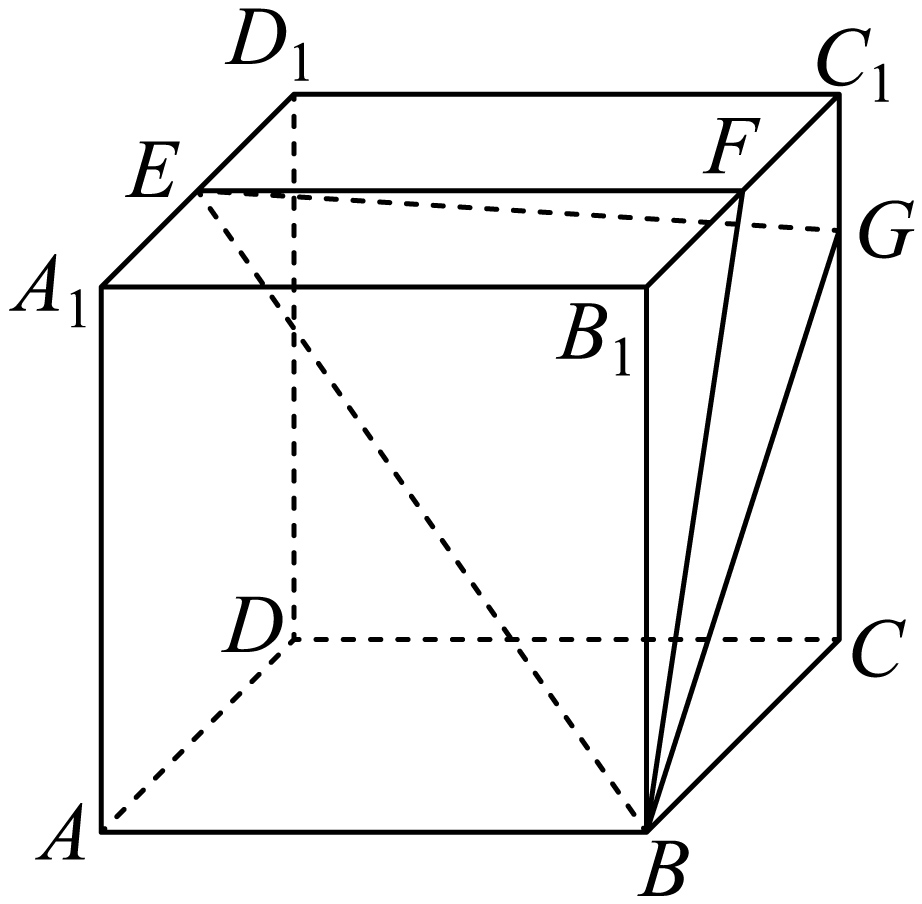
\includegraphics[width=\linewidth]{figures/2025_tj_q17.png}
\end{minipage}

\item（15分）

已知椭圆 $\dfrac{x^2}{a^2}+\dfrac{y^2}{b^2}=1(a>b>0)$ 的左焦点为 $F$，右顶点为 $A$，$P$ 为 $x=a$ 上一点，且直线 $PF$ 的斜率为 $\dfrac13$，$\triangle PFA$ 的面积为 $\dfrac32$，离心率为 $\dfrac12$。

（1）求椭圆的方程；

（2）过点 $P$ 的直线与椭圆有唯一交点 $B$（异于点 $A$），求证：$PF$ 平分 $\angle AFB$。
\newpage
\item（15分）

已知数列 $\{a_n\}$ 是等差数列，$\{b_n\}$ 是等比数列，$a_1=b_1=2$，$a_2=b_2+1$，$a_3=b_3$。

（1）求 $\{a_n\}$，$\{b_n\}$ 的通项公式；

（2）$\forall n\in\mathbb N^*$，$I\in\{0,1\}$，有 $T_n=\{p_1a_1b_1+p_2a_2b_2+\cdots+p_{n-1}a_{n-1}b_{n-1}+p_na_nb_n\mid p_1,p_2,\ldots,p_{n-1},p_n\in I\}$，

（i）求证：对任意实数 $t\in T_n$，均有 $t<a_{n+1}b_{n+1}$；

（ii）求 $T_n$ 所有元素之和。

\item（16分）

已知函数 $f(x)=ax-(\ln x)^2$。

（1）$a=1$ 时，求 $f(x)$ 在点 $(1,f(1))$ 处的切线方程；

（2）$f(x)$ 有 $3$ 个零点，$x_1,x_2,x_3$ 且 $x_1<x_2<x_3$。

（i）求 $a$ 的取值范围；

（ii）证明 $(\ln x_2-\ln x_1)\cdot\ln x_3<\dfrac{4e}{e-1}$。
\end{examanswers}

\end{document}
